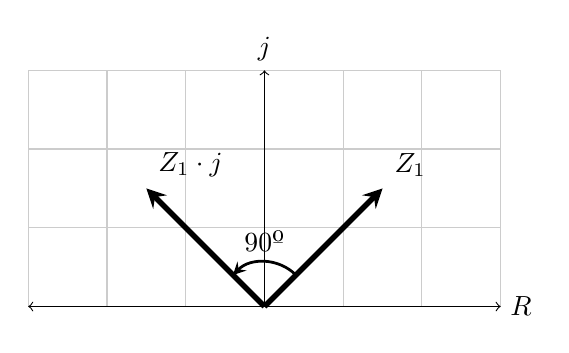
\begin{tikzpicture}
        \draw[thin,gray!40] (-3,0) grid (3,3);
        \draw[<->] (-3,0)--(3,0) node[right] {$R$};
        \draw[<->] (0,0)--(0,3) node[above]{$j$};
        \draw[line width=2pt,black,-stealth](0,0)--(1.5,1.5) node[anchor=south west]{$Z_1$};
        \draw[line width=2pt,black,-stealth](0,0)--(-1.5,1.5) node[anchor=south west]{$Z_1\cdot j$};
        \draw[line width=1pt,black,-stealth] (0.4,0.4) arc (45:135:0.566) node[midway, above]{90º};
\end{tikzpicture}
\caption{Numero complejo multiplicado por la unidad imaginaria}